%10/02/2016 - 
\documentclass[a4 paper, 11  pt]{article}

\usepackage{tabu}  %extended table
\usepackage{ctable}  %extended table
\usepackage{graphicx} %include figures 
\usepackage{epstopdf} %include eps files (transforms eps into pdf)
\usepackage[authoryear,round]{natbib} %style references
\usepackage{amsmath} %mathematical symbols
\usepackage{amssymb} %mathematical symbols 
%\usepackage{bm} %bold mathematical symbols
\usepackage{lineno} %line numbers
\usepackage[colorlinks=true, linkcolor=red, citecolor=blue]{hyperref} %format references - colored and hyperlinked
\usepackage{physics} %for differential d's
\usepackage{rotating}


%\usepackage{etoolbox}
%\AtBeginEnvironment{longtabu}{\footnotesize}{}{}

\textwidth=15.5cm
\textheight=24.0cm
\topmargin=-1cm
\oddsidemargin= 0.2cm
\evensidemargin= 0.2cm
\renewcommand{\topfraction}{0.95}
\renewcommand{\textfraction}{0.05}
\linespread{1.1} 	

\newcommand{\footremember}[2]{%
    \footnote{#2}
    \newcounter{#1}
    \setcounter{#1}{\value{footnote}}%
}
\newcommand{\footrecall}[1]{%
    \footnotemark[\value{#1}]%
} 
\title{Dundee Root Analysis Model (DRAM) - Manual}
\author{%
  G. J. Meijer\footremember{uob}{University of Bath, Department of Arhitecture and Civil Engineering, Bath BA2 7AY, UK (formerly University of Dundee). Email: \href{mailto:gjm36@bath.ac.uk}{gjm36@bath.ac.uk}}%
  }
\date{}

\begin{document}
\maketitle
%\linenumbers

\tableofcontents

%%%%%%%%%%%%%%%%%%%%
%%% INTRODUCTION %%%
%%%%%%%%%%%%%%%%%%%%

%Root-reinforcement calculator - v0.5 - 16/10/2019

\section{Introduction}
This web application was developed by Dr Gerrit Meijer. It provides a user-friendly version of the root-reinforcement model (`Dundee Root Analysis Model', acronym `DRAM') described in full detail by \citet{meijer2019drm}.
This root-reinforcement model accounts for the mobilisation of roots in direct shear conditions, accounting for:
\begin{itemize}
	\parskip=1pt
	\itemsep=0pt
	\item Elastoplastic root behaviour;
	\item  Three-dimensional orientations of roots;
	\item  Root slippage and root breakage mechanisms;
	\item  A shear zone that may increase in thickness during direct shear displacement, depending on the stresses in the soil.
\end{itemize}

The function of this manual is to describe the user interface, and to explain the meaning of all inputs and output. For a detailed explanation of how the root-reinforcement model itself works, please see \citep{meijer2019drm}.

The model runs in `R' \citep{R} and the user interface was created using the `Shiny' package \citep{shiny}. Plots are generated using `Plotly' \citep{plotly}. All plots are interactive, allowing the user to zoom in, zoom out, pan (in 3D plots), switch individual data series on/off, download plots etc.


%%%%%%%%%%%%%
%%% INPUT %%%
%%%%%%%%%%%%%
\section{Input}

This web application uses a simplified set of root and soil input parameters to quickly generate a series of root diameters, orientations etc. The required model input is inputted under several tabs:
\begin{itemize}
	\parskip=1pt
	\itemsep=0pt
	\item \hyperref[sec:inputrootdiameters]{`Root diameters'}: contains input for root diameters and the distribution of root volume fractions over all root diameter classes;
	\item \hyperref[seq:rootorientations]{`Root orientations'}: contains input for generating root orientations;
	\item \hyperref[sec:inputrootproperties]{`Root properties'}: contains input for describing root properties (length, tensile strength, stiffness etc.);
	\item \hyperref[sec:soilproperties]{`Soil properties'}: contains input for soil properties and shear displacements (soil strength, stresses, shear zone thickness, shear displacements etc.).
\end{itemize}
Each of these tabs contains interactive plots \citep[generated using Plotly][]{plotly} that automatically update when input values are changed, to help the user to visualise the input specified. 

In the following, parameters indicated in \textbf{bold} indicate model input parameters.

%%% Unit system
\subsection{Unit system}

The model works with a user-specified system of units, that can be defined on the 'Notes' tab. Units can be set for all:
\begin{itemize}
	\parskip=1pt
	\itemsep=0pt
	\item Length scales (e.g. root diameter, root length, shear displacement, shear zone thickness). Choices are millimeters [mm], centimeters [cm] or meters [m];
	\item Stresses/strengths (e.g. root tensile strength, soil strength and stress, root-reinforcements). Choices are pascals [Pa]=[Nm$^{-2}$], kilopascals [kPa], megapascals [MPa] or gigapascals [GPa].
\end{itemize}
In addition, a root reference diameter $\vb*{d_{r,ref}}$ has to be defined. Such a reference diameter is required for the various power-law relationships used in the model, for example to describe the relation between root diameter and root tensile strength.

All angles are expressed in degrees. 

Please not that when the unit system is \textit{changed} midway using the application, all input parameters of that type are reset to their default values! It is therefore advisable to set the unit system before starting any calculations.

%%% Coordinate system
\subsection{Coordinate system}

Coordinates and angles are expressed in a right-handed coordinate system, orientated in such a way that $x$ points in the direction of shear displacement $u$, and $z$ is normal to the shear plane, pointing in the direction of the displacing soil block, see Figure \ref{fig:coordsystem}. $h$ indicated the current thickness of the shear zone.
\begin{figure}
	\centering
		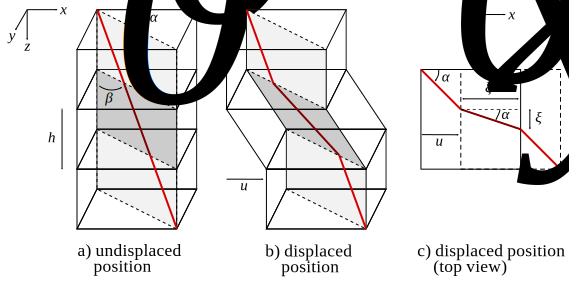
\includegraphics[width=0.8\textwidth]{Figures/20190516_CoordinateSystem.eps}
	\caption{Coordinate system}
	\label{fig:coordsystem}
\end{figure}

The orientation of undisplaced roots is described in spherical coordinates; azimuth $\alpha_0$ (the angle between the $x$ axis and the orientation of the root projected on the $x$-$y$ plane) and elevation angle $\beta_0$ (angle between $z$-axis and root axis). The azimuth and elevation of the displaced root within the shear zone are indicated by $\alpha$ and $\beta$ respectively, see Figure \ref{fig:coordsystem}.

Transverse relative soil--root displacements are assumed zero, i.e. soil and root vectors that are parallel in the undeformed position are assumed to remain parallel in the deformed position. 

%%% Root diameter tab
\subsection{Input tab: `Root diameter'}
\label{sec:inputrootdiameters}

\subsubsection{Root diameter classes}
The range of discrete root diameters can be included in model calculations.
The user defines both the diameter of the smallest root $\vb*{d_{r,min}}$ and the diameter of the largest root $\vb*{d_{r,max}}$. This root diameter interval is split into $\vb*{n_d}$ root diameter classes, each with the same width. The minimum and maximum diameter in each class $i$ ($i=1...n_d$) is given by (Figure \ref{fig:ndiameters}):
\begin{equation}
	d_{r,min,i} = \frac{i-1}{n_d} \qty( d_{r,max}-d_{r,min} )
\end{equation}
\begin{equation}
	d_{r,max,i} = \frac{i}{n_d} \qty( d_{r,max}-d_{r,min} )
\end{equation}
and the average diameter $d_r$ in class $i$:
\begin{equation}
	d_{r,i} = \frac{1}{2} \qty( d_{r,min,i} + d_{r,max,i} )
\end{equation}
\begin{figure}
	\centering
		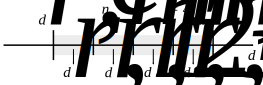
\includegraphics[width=0.5\textwidth]{Figures/20190607_ndiameters.eps}
	\caption{Discretisation of the root diameter range}
	\label{fig:ndiameters}
\end{figure}

\subsubsection{Root volume fractions}
Root volumes are described using root volume fractions, i.e. the fraction of the soil volume occupied by roots. It is assumed that the relationship between root diameter $d_r$ and the root volume fraction described to each root diameter $\phi_r(d_r)$ follows a power-law relationship:
\begin{equation}
	\phi_r(d_r) = a_\phi \qty( \frac{d_r}{d_{r,ref}} )^{b_\phi}
	\label{eq:phirdr}
\end{equation}
where $a_\phi$ and $\vb*{b_\phi}$ are model constants and $d_{r,ref}$ the root reference diameter defined under the `Notes' tab. When $b_\phi=0$, the root volume is equally spread over all root diameters. When $b_\phi>0$, larger roots take up most of the root volume, and when $b_\phi<0$, smaller roots take up the majority of the total root volume, see Figure \ref{fig:rootvolumedistribution}b.

Instead of defining input parameter $a_\phi$, the total root volume fraction $\vb*{\phi_{rt}}$ is defined instead. $a_\phi$ and $\phi_{rt}$ are related since:
\begin{equation}
	\phi_{rt} = \int_{x=d_{r,min}}^{d_{r,max}} \phi_r(x) \dd x
\end{equation}
Rewriting $a_\phi$ in terms of $\phi_{rt}$ gives:
\begin{equation}
	a_\phi = \begin{cases}
	\frac{\phi_{rt} \qty(1+b_\phi)}{d_{r,max}\qty(\frac{d_{r,max}}{d_{r,ref}})^{b_\phi} - d_{r,min}\qty(\frac{d_{r,min}}{d_{r,ref}})^{b_\phi}} & \text{when } b_\phi \neq -1 \\
	\frac{\phi_{rt}}{d_{r,ref} \ln{\qty(\frac{d_{r,max}}{d_{r,min}})}} & \text{when } b_\phi = -1 
	\end{cases}
\end{equation}
\begin{figure}
	\centering
		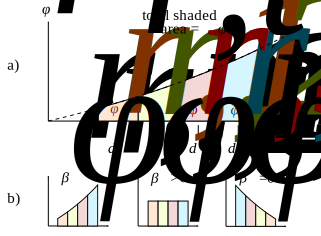
\includegraphics[width=0.6\textwidth]{Figures/20190607_rootfractions.eps}
	\caption{Distribution of root volume fraction over all root diameter classes}
	\label{fig:rootvolumedistribution}
\end{figure}
The root volume fraction that needs to be assigned to each root diameter class $i$ ($\phi_{r,i}$) is found by integrating Equation \ref{eq:phirdr}:
\begin{equation}
	\phi_{r,i} = \int_{x=d_{r,min,i}}^{d_{r,max,i}} \phi_r(d_r) \dd x
\end{equation}


%%% Orientation diameter tab
\subsection{Input tab: 'Root orientations'}
\label{seq:rootorientations}

A range of root orientations can be defined. For every root diameter class, the distribution of root orientations is assumed to be uniform over the range of root orientations specified by the user. 
Initial root orientations are defined in a coordinate system $x'$-$y'$-$z'$ (spherical coordinates: $\alpha'_0$, $\beta'_0$) that is rotated by azimuth angle $\vb*{\alpha_{offset}}$ and elevation angle $\vb*{\beta_{offset}}$ with respect to coordinate system $x$-$y$-$z$, see Figure \ref{fig:orientationoffset}.
\begin{figure}
	\centering
		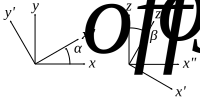
\includegraphics[width=0.5\textwidth]{Figures/20190614_OrientationOffset.eps}
	\caption{Orientation offset of coordinate system used to define initial root orientations}
	\label{fig:orientationoffset}
\end{figure}

The uniform distribution of roots over the specified domain is discretised using $\vb*{n_{ori}}$ discrete root orientation classes. The range of root orientations can either be defined as varying in one dimension ($\vb*{n_{dim}}=1$), two dimensions ($\vb*{n_{dim}}=2$) or three dimensions ($\vb*{n_{dim}}=3$). 

\subsubsection{1-dimensional root orientations}
When the 1-dimensional case is selected ($n_{dim}=1$), only a single root orientation is used with azimuth angle $\alpha'_0=0^\circ$ and elevation angle $\beta'_0=0^\circ$. This root orientation is therefore parallel to the $z'$-axis. Then $n_{dim}=1$ is selected, $n_{ori}$ automatically is assumed to be equal to 1.

\subsubsection{2-dimensional root orientations}
When the 2-dimensional case is selected ($n_{dim}=2$), all roots are orientated in a single 2-D plane spanned by the $x'$ and $z'$-axis, in a `fan' shape around the $z'$-axis . The maximum elevation angle of the fan is given by input parameter $\vb*{\beta'_{0,max}}$. Root orientations are uniformly distributed along this fan, see Figure \ref{fig:2dorientations}. For orientation $i$ ($i=1...n_{ori}$), the azimuth angle $\alpha'_0$ and elevation angle $\beta'_0$ are given by:
\begin{equation}
	\alpha'_{0,i} = 0
\end{equation}
\begin{equation}
	\beta'_{0,i} = \qty[ \frac{2i-1}{n_{ori}} - 1] \beta'_{0,max}
\end{equation}
\begin{figure}
	\centering
		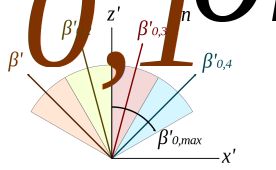
\includegraphics[width=0.4\textwidth]{Figures/20190607_2Drootorientations.eps}
	\caption{2-dimensional root orientations ($n_{dim}=2$), using $n_{ori}=4$ and $\beta'_{0,max}=60^\circ$.}
	\label{fig:2dorientations}
\end{figure}

\subsubsection{3-dimensional root orientations}
When the 3-dimensional case is selected ($n_{dim}=3$), roots are orientated in three dimensional space. Root orientations are assumed uniformly distributed over a spherical cap, described by the domain $-180^\circ \leq \alpha'_0 < 180^\circ$ and $0 \leq \beta'_0 \leq \beta'_{0,max}$. This domain is discretised in the following manner:
\begin{enumerate}
	\parskip=1pt
	\itemsep=0pt
	\item Define a rectangular grid with $n_{row}$ rows and $n_{col}$ columns, on the cartesian domain $-\beta'_{0,max} \leq x^* \leq \beta'_{0,max}$, $-\beta'_{0,max} \leq y^* \leq \beta'_{0,max}$, see Figure \ref{fig:polargrid}a. The number of rows and columns is calculated as:
		\begin{equation}
		 n_{col} = \text{ceiling}\qty(\sqrt{n_{ori}})
		\end{equation}
		\begin{equation}
			n_{row} = \text{ceiling}\qty(\frac{n_{ori}}{n_{col}})
		\end{equation}
	\item Transform this grid into a polar grid by scaling the grid into a circular shape with radius $\beta'_{0,max}$ (Figure \ref{fig:polargrid}b). New $x^{**}$ and $y^{**}$ positions are found by dividing the $x^*$ and $y^*$ positions by the length of the vector that originates in (0,0), passes through ($x^*$,$y^*$) and ends on the edge of the grid;
	\item In this new polar grid, the distance between a point and the origin is the root elevation angle $\beta'_{0}$, and the angle between the point position vector and the $x^{**}$ axis is equal to the root azimuth angle $\alpha'_0$, see Figure \ref{fig:polargrid}b;
	\item Use the midpoints of each grid cell as the discrete root orientations ($\alpha'_0$, $\beta'_0$) in the model;
	\item Calculate the area of each deformed grid cell in the spherical cap (each cell might have a slightly different area due to the transformation to a polar grid) and divide over the area of the spherical cap to calculate the relative root volume fraction that needs to be assigned to each discrete root orientation.
\end{enumerate}
Note that due to this procedure, the actual number of discrete root orientations used may be slightly larger than the number of requested root orientations ($n_{row} n_{col} \geq n_{ori}$).
\begin{figure}
	\centering
		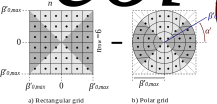
\includegraphics[width=0.80\textwidth]{Figures/20191016_PolarGrid.eps}
	\caption{Procedure to gain a discrete number of root orientations in three dimensions ($n_{ori}=3$). Plotted is the grid used when selecting $ 31 \leq n_{ori} \leq 36$ discrete root orientations}
	\label{fig:polargrid}
\end{figure}

%%% Root properties
\subsection{Input tab: `Root properties'}
\label{sec:inputrootproperties}

On this input tab, root properties such as root length and their biomechanical behaviour are defined.

The root tensile strength $t_{ru}$ is modelled as varying as function of root diameter $d_r$ by means of a power-law function:
\begin{equation}
	t_{ru}(d_r) = a_t \qty(\frac{d_r}{d_{r,ref}})^{b_t}
	\label{eq:tru}
\end{equation}
where $\vb*{a_t}$ is the tensile strength of roots with a diameter $d_r=d_{r,ref}$, $\vb*{b_t}$ a dimensionless power coefficient. Although often ignored, the reference diameter $d_{r,ref}$ should always be specified to maintain a consistent system of units. The magnitude of the root reference diameter is set under the `Notes' tab.

Another power-law function is used to describe the tensile strain to failure $\epsilon_{ru}$ as function of root diameter $d_r$:
\begin{equation}
	\epsilon_{ru}(d_r) = a_\epsilon \qty(\frac{d_r}{d_{r,ref}})^{b_\epsilon}
	\label{eq:eru}
\end{equation}
where $\vb*{a_\epsilon}$ is the tensile strain to failure of roots with a diameter $d_r=d_{r,ref}$, and $\vb*{b_\epsilon}$ a dimensionless power coefficient.

Similarly, a power-law is used to describe the root length $L_r$ as function of root diameter $d_r$:
\begin{equation}
	L_r(d_r) = a_L \qty(\frac{d_r}{d_{r,ref}})^{b_L}
\end{equation}
where $\vb*{a_L}$ is the root length of roots with a diameter $d_r=d_{r,ref}$, and $\vb*{b_L}$ a dimensionless power coefficient.

Roots are modelled as elastoplastic, where $t_{ry}$ is the yield tensile strength and $\epsilon_{ry}$ the yield tensile strain, see Figure \ref{fig:tensilestressstrain}. The (elastic) Young's modulus $E_{re}$ equals:
\begin{equation}
	E_{re} = \frac{t_{ry}}{\epsilon_{ry}}
	\label{eq:ere}
\end{equation}
and the elastoplastic stiffness $E_{rep}$:
\begin{equation}
	E_{rep} = \frac{t_{ru} - t_{ry}}{\epsilon_{ru} - \epsilon_{ry}} 
	\label{eq:erep}
\end{equation}
The yield tensile stress $t_{ry}$ and yield strain $\epsilon_{ry}$ are inputted in the model as fractions of tensile strength $t_{ru}$ and tensile strain to failure $\epsilon_{ru}$ respectively, using (dimensionless) parameters $\vb*{t_{ry}/t_{ru}}$ and $\vb*{\epsilon_{ry}/\epsilon_{ru}}$.
\begin{figure}
	\centering
		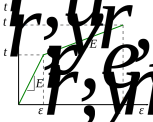
\includegraphics[width=0.5\textwidth]{Figures/20190527_ElastoPlasticRoot_Definitions.eps}
	\caption{Root elastoplastic tensile stress-strain behaviour incorporated in the model.}
	\label{fig:tensilestressstrain}
\end{figure}

The evolution of root tensile stress as function of tensile strain, ignoring any root breakage effects, can be described as:
\begin{equation}
	t_{ri}(\epsilon_r) = 
	\begin{cases}
		E_{re} \epsilon_r & \text{when } \epsilon_r \leq \epsilon_{ry} \\
		t_{ry} + E_{rep} \qty(\epsilon_r - \epsilon_{ry}) & \text{when } \epsilon_r > \epsilon_{ry}
	\end{cases}
	\label{eq:tri}
\end{equation}

After substitution of Equations \ref{eq:tru} and \ref{eq:eru} into Equations \ref{eq:ere} and \ref{eq:erep}, it follows that the elastic and elastoplastic root stiffnesses $E_{re}$ and $E_{rep}$ can be rewritten in terms of root diameter $d_r$ using a power law relationship:
\begin{equation}
	E_{re}(d_r) = \frac{\qty(t_{ry}/t_{ru})}{\qty(\epsilon_{ry}/\epsilon_{ru})} \frac{a_t}{a_\epsilon} \qty(\frac{d_r}{d_{r,ref}})^{b_t - b_\epsilon}
\end{equation}
\begin{equation}
	E_{re}(d_r) = \frac{\qty(1 - t_{ry}/t_{ru})}{\qty(1 - \epsilon_{ry}/\epsilon_{ru})} \frac{a_t}{a_\epsilon} \qty(\frac{d_r}{d_{r,ref}})^{b_t - b_\epsilon}
\end{equation}

It is known that the biomechanical properties of roots can vary widely, not only between roots with different diameters, but also for roots with the \textit{same} diameter. To include the latter variability in the model, a root breakage parameter $f_{break}$ was included, such that $f_{break}=1$ when all root is intact, and $f_{break}=0$ when all root is broken. The average tensile stress $\bar{t}_r$ in all roots with diameter $d_r$ as function of tensile strain $\epsilon_r$ is given by:
\begin{equation}
	\bar{t}_r(\epsilon_r) = f_{break} t_{ri}(\epsilon_r)
\end{equation}
The Weibull breakage function is used to define the breakage parameter $f_{break}$, similar to \citet{schwarz2013}:
\begin{equation}
	f_{break} = -\exp \qty[-\qty( \frac{t_{ri}}{\lambda_t} )^{\kappa_t} ]
\end{equation}
where $\kappa_t$ is the (dimensionless) Weibull shape parameter and $\lambda_t$ the (dimensionless) Weibull scale parameter, which is related to the average root strength $t_{ru}$:
\begin{equation}
	\lambda_t = \frac{t_{ru}}{\Gamma(1 + 1/\kappa_t)}
	\label{eq:weibullshaperelation}
\end{equation}
where $\Gamma$ is the Gamma-function.

If elastic root behaviour is required in the model instead of elastoplastic root behaviour, simply ensure that input parameters $t_{ry}/t_{ru} = \epsilon_{ry}/\epsilon_{ru}$. 


%%%
\subsection{Input tab: `Soil properties'}
\label{sec:soilproperties}

On this input tab, soil properties, root-soil interface properties, shear zone properties and direct shear displacements are defined. 

The soil shear strength $\tau_s$ is described using the Mohr-Coulomb failure criterion:
\begin{equation}
	\tau_s = c + \sigma'_n \tan\phi'
\end{equation}
where $\vb*{c}$ is the soil cohesion, $\vb*{\phi'}$ the soil angle of internal friction and $\vb*{\sigma'_n}$ the soil effective normal stress acting on the shear zone (positive in compression).

The maximum root--soil interface friction is described by $\vb*{\tau_i}$. Full interface friction between soil and root is assumed in the model as soon as there is differential displacement between soil and root (rigid perfectly-plastic behaviour).

The initial thickness $h$ of the shear zone is inputted into the model through model parameter $\vb*{h_0}$. In geotechnical engineering, this is often assumed in the order of 10 to 20 average soil particle diameters \citep[e.g.][]{oda1999}. A maximum shear zone thickness $\vb*{h_{max}}$ can also be specified, for example when modelling a case where the shear zone thickness may be limited by boundary conditions. If there is no constraint, simply set $h_{max}$ equal to a large value.

The maximum direct shear deformation $u$ applied in the model is described by parameter $\vb*{u_max}$. The shear displacement interval is split into $\vb*{n_step}$ number of uniformly spaced shear displacement steps. The shear displacement in step $i$ ($i=1...n_{step}$) is given by:
\begin{equation}
	u_i = \frac{i}{n_{step}} u_{max}
\end{equation}

It should be noted that the case $h = h_0 = h_{max} = 0$ is equivalent with modelling the opening of a tensile crack, for example at the crown of a landslide. In this case, $u$ now signifies the crack width, and $u_{max}$ the maximum crack width considered.


%%%%%%%%%%%%%%
%%% OUTPUT %%%
%%%%%%%%%%%%%%

\section{Output}

Output is provided on two output tabs:
\begin{itemize}
	\parskip=1pt
	\itemsep=0pt
	\item \hyperref[sec:outputdrm]{`Calculate'}: On this tab, calculations using the Dundee Root Model are performed and the results plotted; 
	\item \hyperref[sec:outputdrm]{`Comparison to existing models'}: On this tab, root-reinforcements are calculated using other existing root-reinforcement models (using the same input parameters as used in the DRAM).
\end{itemize}

%%% DRM
\subsection{Output tab: 'Calculate'}
\label{sec:outputdrm}
Calculations for the Dundee Root Model are started by pressing the button `Start calculations'.
Calculation progress is indicated in the lower-right corner of the screen.
Once finished, three (interactive) plots will appear:
\begin{enumerate}
	\parskip=1pt
	\itemsep=0pt
	\item Shear displacement--root reinforcement plot: Plots the calculated root-reinforcement $c_r$ as function of direct shear displacement $u$, as calculated by the DRAM. The peak root-reinforcements $c_{ru}$ and the corresponding shear displacement are indicated on the plot. The 'WWM-coefficient' indicates the corresponding multiplication factor $k'$ that should be used in the Wu/Waldron model to obtain the same value of $c_r$ as found by the DRAM;
	\item Shear displacement--shear zone thickness plot: Plots the evoluation of the thickness of the shear zone ($h$) as function of shear displacement ($u$);
	\item Shear displacement--root fraction plot. This stacked area plot indicates the fractions of the total root volume of roots behaving elastic, elastoplastic, anchored, slipping, broken etc., as function of shear displacement $u$. This plots should give some insight of what the dominant type of root behaviour is throughout the test.
\end{enumerate}
In addition, two comma-separated data files (\texttt{.csv}) can be downloaded:
\begin{enumerate}
	\parskip=1pt
	\itemsep=0pt
	\item Input: Contains a list of all input parameters, units and values fed into the model:
		\begin{itemize}
		\parskip=0pt
		\itemsep=0pt
		\item \texttt{phirt}: total root volume fraction $\phi_{rt}$
		\item \texttt{bphi}: root volume distribution power coefficient $b_\phi$
		\item \texttt{nd}: number of discrete root diameters $n_d$
		\item \texttt{drmin}: minimum root diameter $d_{r,min}$
		\item \texttt{drmax}: mazimum root diameter $d_{r,min}$
		\item \texttt{nori\_requested}: requested number of discrete root orientations $n_{ori}$
		\item \texttt{nori\_usedinmodel}: number of discrete root orientations used by the model
		\item \texttt{ndim}: number of root orientation dimension $n_{dim}$
		\item \texttt{beta0max}: maximum root elevation angle $\beta'_{0,max}$, in $x'$-$y'$-$z'$ coordinate system
		\item \texttt{alpha0offset}: azimuth angle offset $\alpha_{offset}$ between $x'$-$y'$-$z'$ and $x$-$y$-$z$ coordinate systems
		\item \texttt{beta0offset}: elevation angle offset $\beta_{offset}$ between $x'$-$y'$-$z'$ and $x$-$y$-$z$ coordinate systems
		\item \texttt{drref}: reference root diameter $d_{r,ref}$
		\item \texttt{at}: root tensile strength $a_t$ for roots with diameter $d_r=d_{r,ref}$
		\item \texttt{bt}: root diameter--tensile strength power coefficient $b_t$
		\item \texttt{aepsilon}: root tensile strain to failure $a_\epsilon$ for roots with diameter $d_r=d_{r,ref}$
		\item \texttt{bepsilon}: root diameter--tensile strain to failure power coefficient $b_\epsilon$
		\item \texttt{aL}: root length $a_L$ for roots with diameter $d_r=d_{r,ref}$
		\item \texttt{bL}: root diameter--root length power coefficient $b_L$
		\item \texttt{trytru}: ratio $t_{ry}/t_{ru}$ between root yield strength and tensile strength
		\item \texttt{eryeru}: ratio $\epsilon_{ry}/\epsilon_{ru}$ between root yield strain and strain to failure
		\item \texttt{c}: soil cohesion $c'$
		\item \texttt{phi}: soil angle of internal friction $\phi'$
		\item \texttt{sign}: effective normal soil stress $\sigma'_n$ on the shear plane 
		\item \texttt{h0}: initial shear zone thickness $h_0$
		\item \texttt{hmax}: maximum shear zone thickness $h_{max}$
		\item \texttt{taui}: maximum root--soil interface friction $\tau_i$
		\item \texttt{umax}: maximum shear displacement $u_{max}$ considered in the model
		\item \texttt{nstep}: number of discrete shear displacement steps $n_{step}$
		\end{itemize}
	\item Output: Contains the data underlying the three plots shown. The output file contains the following columns:
	\begin{itemize}
		\parskip=0pt
		\itemsep=0pt
		\item \texttt{StepID}: Integer indicating the number of the current shear displacement step;
		\item \texttt{u}: Current direct shear displacement $u$;
		\item \texttt{h}: Current shear zone thickness $h$;
		\item \texttt{cr}: Current root-reinforcement $c_r$;
		\item \texttt{WWMfactor}: Current equivalent Wu/Waldron factor $k'$, i.e. the WWM multiplication factor that is required to match the peak root-reinforcement calculated using the DRAM;
		\item \texttt{Fraction\_NotInTension}: The fraction of the total root volume of roots currently not loaded in tension or fully positioned within the shear zone;
		\item \texttt{Fraction\_AnchoredElastic}: The fraction of the total root volume of roots that currently behave anchored and linear elastic;
		\item \texttt{Fraction\_AnchoredElastoplastic}: The fraction of the total root volume of roots that currently behave anchored and elastoplastic;
		\item \texttt{Fraction\_SlippingElastic}: The fraction of the total root volume of roots that currently slip and behave linear elastic;
		\item \texttt{Fraction\_SlippingElastoplastic}: The fraction of the total root volume of roots that currently slip and behave elastoplastic;
		\item \texttt{Fraction\_Broken}: The fraction of the total root volume of roots that are currently broken;
	\end{itemize}
	This file can only be downloaded after the calculations have finished.
\end{enumerate}


%%% Other models
\subsection{Output tab: `Comparison to existing models'}
\label{sec:existingmodels}

On this tab, root-reinforcement is calculated using existing models:
\begin{itemize}
	\parskip=1pt
	\itemsep=0pt
	\item \hyperref[sec:wwm]{Wu/Waldron model (WWM)}
	\item \hyperref[sec:fbm]{Fibre bundle model (FBM)}
	\item \hyperref[sec:rbm]{Root Bundle Model (RBM)}
	\item \hyperref[sec:rbm]{Root Bundle Model with weibull curves (RBMw)}
\end{itemize}
These models are described in the following sections.

%%% wwm
\subsubsection{Wu/Waldron model (WWM)}
\label{sec:wwm}
The peak root-reinforcement $c_{ru}$, according to the Wu/Waldron model (`WWM'), is found by summing the contributions of all roots $i$ \citep{waldron1977,wu1979}:
\begin{equation}
	c_{ru} = k' \sum_i \phi_{r,i} t_{ru,i}
\end{equation}
Where $k'$ is a user defined multiplication factor, $\phi_{r,i}$ the root volume fraction (or root area ratio) for root $i$, and $t_{ru,i}$ the tensile strength of root $i$

This model assumes that all root break simultaneously in tension, and therefore provides an upper limit to calculated root-reinforcements. This model is known to significantly overestimate peak root reinforcements.

%%% fbm
\subsubsection{Fibre bundle model (FBM)}
\label{sec:fbm}
Fibre Bundle Models (`FBM') have been used to address progressive breakage of roots \citep{pollen2005}. In these models, the total tensile load in a bundle of roots $F = A_s c_{ru}/k'$ (i.e. total root tensile force over a shear plane with area $A_s$) is distributed among all intact roots. An important modelling choice is how to distribute the load over roots, given the variation in their properties. This is often based on some rule involving the root diameter $d_r$. The tensile force in intact root $i$ ($F_i$) can be described by:
\begin{equation}
	\frac{F_i}{d_{r,i}^a} = \frac{F}{\sum\limits_{j=1}^{n} d_{r,j}^a}
	\label{eq:fbmloadsharing}
\end{equation}
where $a$ is a model constant, and $n$ the number of intact roots. Once the tensile force exceeds the strength in a root, it breaks and the load it carried is distributed over remaining intact roots. Incrementally increasing the load until all roots have failed yields the maximum force the bundle can sustain, and thus the maximum root-reinforcement $c_{ru}$:
\begin{equation}
	c_{ru} = k' \frac{\max F}{A_s}
\end{equation}
Where $k'$ again is the Wu/Waldron multiplication coefficient, included to account for the influence of root orientations. 

Common choices of $a$ are $a=0$ (load is equally distributed over all roots, regardless of the diameter), $a=1$ (load is split proportional to root diameters) and $a=2$ (resulting in equal stresses in all roots) \citep[see for example][]{comino2010,thomas2010,mao2012}. There is however no reason why other values of $a$ cannot be used, and the FBM incorporated here allows any value of $a$ to be specified.

A plot with the FBM output is generated, showing the calculated root-reinforcement as function of the diameter of the currently breaking root. Arrows indicate the order of root breakage. Peak reinforcements $c_{ru}$ are indicated using plot annotations.

\subsubsection{Root Bundle Models (FBM/FBMw)}
\label{sec:rbm}

The Root Bundle Model' (`RBM'), an alternative fibre bundle approach, was developed by \citet{schwarz2010}, distributing the tensile load over a bundle of roots according to the root stiffness. The model assumes a bundle of parallel roots with equal tensile strain $\epsilon_r$ in all roots. 

In the original Schwarz et al. papers, linear elastic roots were assumed, but to stay in line with the Dundee Root Model, elastoplastic root behaviour was incorporate in the RBM included in this application, according to Equation \ref{eq:tri}.

Root breakage is incorporated using a breakage parameter $f_{break}$,  indicating whether roots are intact ($f_{break}=1$) or broken ($f_{break}=0$). The (average) root tensile strength, including root breakage, now equals:
\begin{equation}
	\bar{t}_r(\epsilon_r) = f_{break} t_{ri}(\epsilon_r)
\end{equation}
In the case where roots suddenly break (as in the original RBM), $f_{break}=1$ when $\epsilon_r \leq \epsilon_{ru}$ and $f_{break}=0$ when $\epsilon_r > \epsilon_{ru}$, i.e.:
\begin{equation}
	f_{break}(\epsilon_r) = H(\epsilon_{ru} - \epsilon_{r})
\end{equation}
where $H$ is the Heaviside function ($H(x<0)=0$, $H(x\geq0)=1$).

In a later model version by \citet{schwarz2013} with the acronym `RBMw', root failure was `smoothed' using a Weibull survival function, accounting for progressive root failure within the root diameter class:
\begin{equation}
	f_{break}(\epsilon_r) = \exp \qty( - \qty[ \frac{t_{ri}(\epsilon_r)}{\lambda_t} ]^{
	\kappa_t} )
\end{equation}
where $\lambda_t$ and $\kappa_t$ are the Weibull scale and shape parameter describing the probability distribution of root tensile strength $t_{ru}$ within the root diameter class, and $t_{ri}$ the tensile strength in the (infinitely strong) root, see Equation \ref{eq:tri}). Shape parameter $\kappa_t$, scale parameter $\lambda_t$ and the average root strength $t_{ru}$ can be related to each other through Equation \ref{eq:weibullshaperelation}.

At a given tensile strain $\epsilon_r$, the current root reinforcement equals:
\begin{equation}
	c_{r}(\epsilon_r) = k' \sum_i \phi_{r,i} \bar{t}_{r,i}(\epsilon_r) 
\end{equation}
And therefore the peak root reinforcement $c_{ru}$ can be found by finding the maximum of $c_{r}(\epsilon_r)$ on the domain $\epsilon_r \geq 0$.
\begin{equation}
	c_{ru} = k' \max \qty( \sum_i \phi_{r,i} \bar{t}_{r,i}(\epsilon_r)  )
\end{equation}

A plot with the RBM and RBMw output, plotting root-reinforcement $c_r$ as function of tensile strain $\epsilon_r$. Peak reinforcements $c_{ru}$ and the tensile strain at which these occur are indicated using plot annotations.


%%%%%%%%%%%%%%%%%%%%%%%%%%%
%% BIBLIOGRAPHY
%%%%%%%%%%%%%%%%%%%%%%%%%%%

\addcontentsline{toc}{section}{Bibliography}
\bibliographystyle{plainnat} 
\bibliography{References_BibTeX}


\end{document}